\documentclass[dvipdfmx]{beamer}

\usepackage{beamerthemesplit}
\usepackage[]{graphicx}
\graphicspath{%
{./slide07-img/}%
{./text07-img/}%
}

\usepackage{listings}
\usepackage{hyperref}
\usepackage{pxjahyper}
\usepackage{nameref} % これが\zexternaldocumentの前までに必要
\usepackage{zref-xr}
\usepackage{color}

\zxrsetup{toltxlabel} % 通常のLaTeXスタイルの\refを使う(\zexternaldocumentより前におく)
\zexternaldocument*[1:]{text07} % \zのついたexternaldocumentを使う

\setbeamertemplate{footline}[frame number]
\title{子どもIT未来塾 第7回}
\author{塾長 清水尚彦}

\def\quiz{1}

\begin{document}

\frame{
   \begin{center}
    \huge{子どもIT未来塾}\\

    \vspace{48pt}
	   \Large{第7回}\\
	   {\huge\bf ネットワークについて学ぼう}\\
    \vspace{24pt}
    \large{塾長 清水尚彦}\\
    \vspace{10pt}
    \large{\the\year 年 9月23日}
  \end{center}
}



\begin{frame}[fragile]
	\frametitle{2時間目 みんなで自己紹介ページを見よう ~~~\raisebox{-3mm}{
\includegraphics[width=0.1\textwidth]{raspberry}}}
    \large\textbf{ウェブサーバを立ち上げて、自分のホームページを公開しよう}
        \begin{itemize}
            \item みんなの自己紹介ページをネットワークを使って見てみよう
        \end{itemize}
        \begin{minipage}{\textwidth}
            {\upshape
              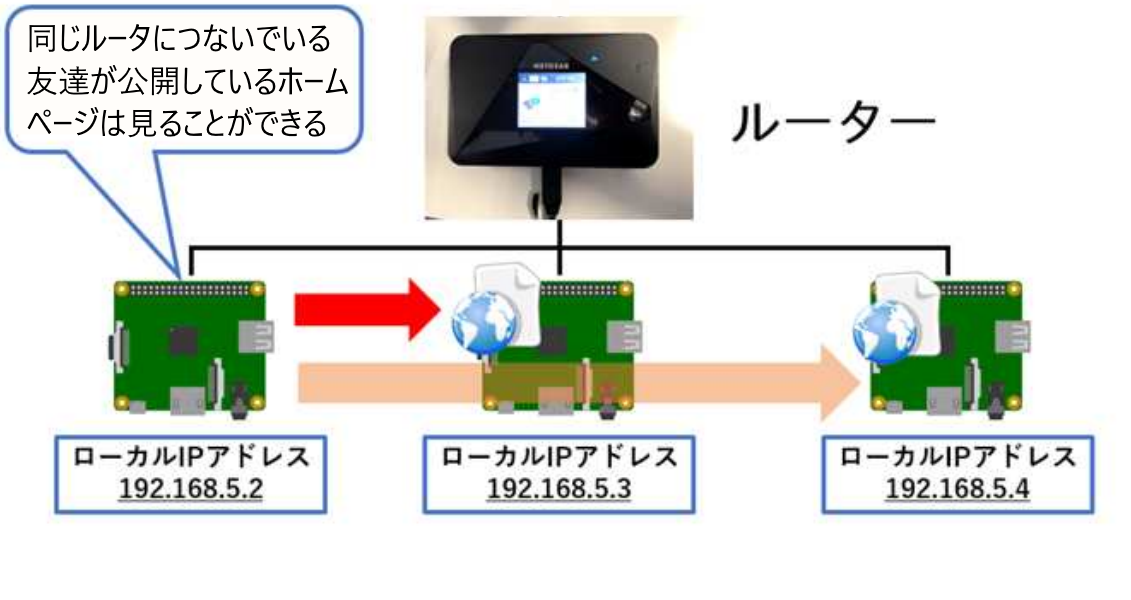
\includegraphics[width=\textwidth]{slide07-img015.png}}
        \end{minipage}
\end{frame}

\begin{frame}[fragile]
	\frametitle{HTMLを復習しよう:テキスト P.\pageref{1:P:HTML}-.\pageref{1:P:HP}~~~\raisebox{-3mm}{
\includegraphics[width=0.1\textwidth]{raspberry}}}
      \large\textbf{教科書をよみながら、問題をやってみよう}
				\begin{itemize}
					\item \ref*{1:E:HTML}
					\item \ref*{1:Q:HTML} 
				\end{itemize}
      \vfill
      \large\textbf{わからないことは、放っておかず、すぐに TA に聞きましょう}
\end{frame}

\begin{frame}[fragile]
	\frametitle{ウェブサーバを立ち上げよう:テキスト P.\pageref{1:P:HP}-P.\pageref{1:P:CGI}~~~\raisebox{-3mm}{
\includegraphics[width=0.1\textwidth]{raspberry}}}
    \large\textbf{クライアントとサーバについて知ろう}\\
			\begin{minipage}{\textwidth}
                {\upshape
                  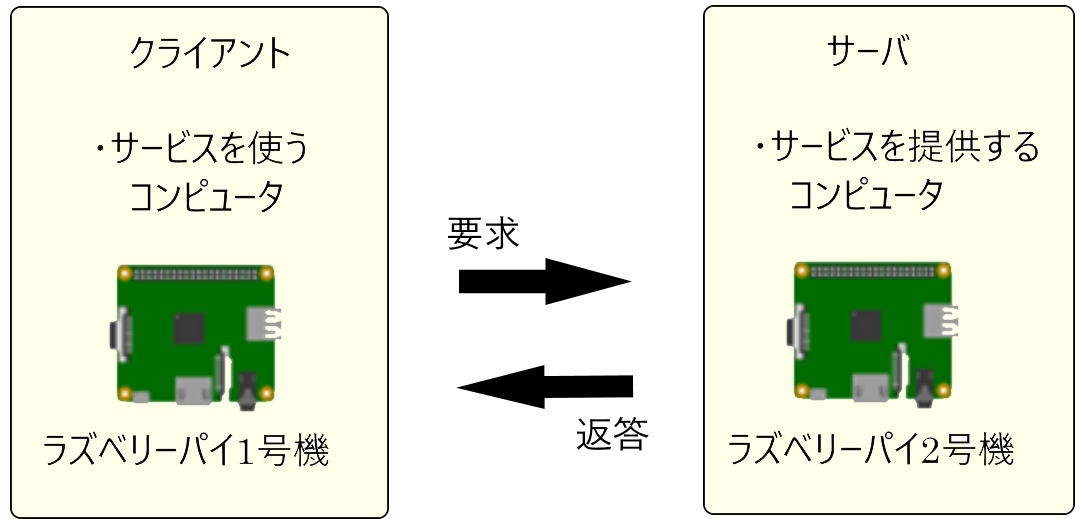
\includegraphics[width=\textwidth]{slide07-img014.png}}
            \end{minipage}
            \begin{itemize}
                \item クライアントとサーバーは同じコンピュータにあっても問題ありません。
            \end{itemize}
\end{frame}

\begin{frame}[fragile]
	\frametitle{ウェブサーバを立ち上げよう:テキスト P.\pageref{1:P:HP}-P.\pageref{1:P:CGI}~~~\raisebox{-3mm}{
\includegraphics[width=0.1\textwidth]{raspberry}}}
            \begin{itemize} 
                \item 違うルータに接続している子のIPアドレスを入力しても、アクセスすることはできません。
            \end{itemize}
			\begin{minipage}{\textwidth}
                {\upshape
                  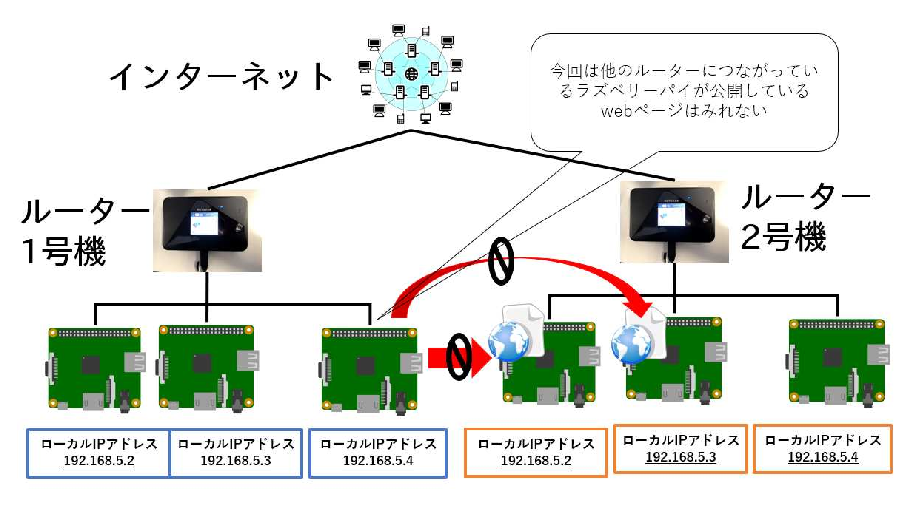
\includegraphics[width=\textwidth]{ome7-img045}}
            \end{minipage}
\end{frame}

\begin{frame}[fragile]
	\frametitle{ウェブサーバを立ち上げよう:テキスト P.\pageref{1:P:HP}-P.\pageref{1:P:CGI}~~~\raisebox{-3mm}{
\includegraphics[width=0.1\textwidth]{raspberry}}}
      \large\textbf{教科書をよみながら、問題をやってみよう}
				\begin{itemize}
					\item \ref*{1:E:myHP}
					\item \ref*{1:friend} 
					\item \ref*{1:Q:otherHP} 
				\end{itemize}
      \vfill
      \large\textbf{わからないことは、放っておかず、すぐに TA に聞きましょう}
\end{frame}

\end{document}
